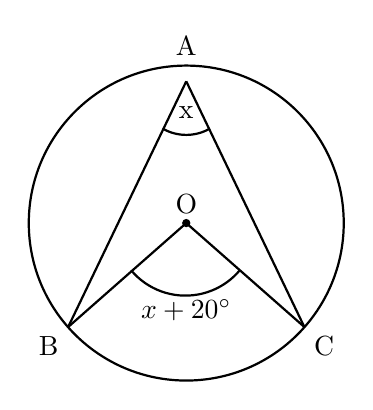
\begin{tikzpicture}[scale=1]

  % Define the center of the circle
  \coordinate (O) at (0,0);

  % Define the radius of the circle
  \def\R{2}

  % Draw the circle
  \draw[thick] (O) circle (\R);

  % Add a dot at the center
  \fill (O) circle (1.5pt);

  % Add the label 'O' near the center
  \node[above] at (O) {O};

  % Define coordinates for points A, B, and C
  % A is near the top
  \coordinate (A) at (0, 1.8);
  % B and C are near the bottom
  \coordinate (B) at (-1.5, -1.32);
  \coordinate (C) at (1.5, -1.32);

  % Draw the lines connecting A, B, and C
  \draw[thick] (A) -- (B);
  \draw[thick] (A) -- (C);

  % Draw the lines from the center O to B and C
  \draw[thick] (O) -- (B);
  \draw[thick] (O) -- (C);

  % Add labels for the points A, B, and C
  \node[above] at (0, 2) {A};
  \node[below left] at (B) {B};
  \node[below right] at (C) {C};

  % Draw arc for angle at A (x)
  \draw[thick] (-0.3, 1.2) arc (240:300:0.6);
  \node at (0, 1.4) {x};

  % Draw arc for angle at O (x+20°)
  \draw[thick] (-0.7, -0.6) arc (220:320:0.9);
  \node at (0, -1.1) {$x+20^{\circ}$};

\end{tikzpicture}